\section{19th March 2023: Truth about Judgment and Salvation}
\subsection*{Text: Revelation 14:1-20}
  \begin{quote}
    [1] Then I looked, and behold, on Mount Zion stood the Lamb, and with him
    144,000 who had his name and his Father’s name written on their
    foreheads.  [2] And I heard a voice from heaven like the roar of many
    waters and like the sound of loud thunder.  The voice I heard was like
    the sound of harpists playing on their harps, [3] and they were singing a
    new song before the throne and before the four living creatures and
    before the elders.  No one could learn that song except the 144,000 who
    had been redeemed from the earth.  [4] It is these who have not defiled
    themselves with women, for they are virgins.  It is these who follow the
    Lamb wherever he goes.  These have been redeemed from mankind as
    firstfruits for God and the Lamb, [5] and in their mouth no lie was
    found, for they are blameless.

    [6] Then I saw another angel flying directly overhead, with an eternal
    gospel to proclaim to those who dwell on earth, to every nation and tribe
    and language and people.  [7] And he said with a loud voice, “Fear God
    and give him glory, because the hour of his judgment has come, and
    worship him who made heaven and earth, the sea and the springs of water.”

    [8] Another angel, a second, followed, saying, “Fallen, fallen is Babylon
    the great, she who made all nations drink the wine of the passion of her
    sexual immorality.”

    [9] And another angel, a third, followed them, saying with a loud voice,
    “If anyone worships the beast and its image and receives a mark on his
    forehead or on his hand, [10] he also will drink the wine of God’s wrath,
    poured full strength into the cup of his anger, and he will be tormented
    with fire and sulfur in the presence of the holy angels and in the
    presence of the Lamb.  [11] And the smoke of their torment goes up
    forever and ever, and they have no rest, day or night, these worshipers
    of the beast and its image, and whoever receives the mark of its name.”

    [12] Here is a call for the endurance of the saints, those who keep the
    commandments of God and their faith in Jesus.

    [13] And I heard a voice from heaven saying, “Write this: Blessed are the
    dead who die in the Lord from now on.” “Blessed indeed,” says the Spirit,
    “that they may rest from their labors, for their deeds follow them!”

    [14] Then I looked, and behold, a white cloud, and seated on the cloud
    one like a son of man, with a golden crown on his head, and a sharp
    sickle in his hand.  [15] And another angel came out of the temple,
    calling with a loud voice to him who sat on the cloud, “Put in your
    sickle, and reap, for the hour to reap has come, for the harvest of the
    earth is fully ripe.” [16] So he who sat on the cloud swung his sickle
    across the earth, and the earth was reaped.

    [17] Then another angel came out of the temple in heaven, and he too had
    a sharp sickle.  [18] And another angel came out from the altar, the
    angel who has authority over the fire, and he called with a loud voice to
    the one who had the sharp sickle, “Put in your sickle and gather the
    clusters from the vine of the earth, for its grapes are ripe.” [19] So
    the angel swung his sickle across the earth and gathered the grape
    harvest of the earth and threw it into the great winepress of the wrath
    of God.  [20] And the winepress was trodden outside the city, and blood
    flowed from the winepress, as high as a horse’s bridle, for 1,600 stadia.
  \end{quote}
\subsection*{Notes}
\begin{itemize}
  \item{This chapter gives us a preview of the end times. And this is to encourage the believers in the battle against the evil one.}
  \item{Three points today: 
  \begin{itemize}
    \item{Encouragement for the redeemed.}
    \item{The message.}
    \item{Judgment of the rebels.}
  \end{itemize}}
  \item{From the first point, we see the $144000$ are the ones who are
  standing with Mt Zion with the Lamb, they sing a new song, they are not
  defiled, and bear the mark/seal of the Lamb, and they are followers of the
  Lamb.  These $144000$ are also singing a song that nobody else could learn.
  This makes sense because its like the world doesn't understand the gospel
  message, it is foolishness to the Jew and the Greek.}
  \item{ These $144000$ are a symbol for the people of God, and if we recall
  from the previous sermon, if we take the $144000$ to be the Church militant
  on earth (i.e the Church on earth who is still fighting against the powers
  of darkness), then the phraseology ``have not defiled themselves with
  women'' is a throwback to how in the OT the fighting men were not supposed
  to have relations with women.  Hence, when this phraseology is applied to
  the $144000$, then it means that the $144000$ are both pure and ready for
  war.  But even though the $144000$ are preparing for war with evil, they
  are also kept secure by God and the Lamb, through the seal that is put on
  them.  These $144000$ are also the firstfruits for God and the Lamb, which
  is a reference to how they have been dedicated to God.  }
  \item{From the second point, the good news here (gospel) is about how God's
  kingdom is now established for all eternity, and that judgment is coming on
  the earthly sinful kingdoms who carry out injustice (and this is all
  earthly kingdoms btw).  This would be good news to those who await the
  coming of God and hence are oppressed for that.}
  \item{But for those who are part of the earthly sinful kingdoms, of which
  Babylon is an archetype, this gospel is bad news (unless they repent).  The
  news is this; because of God's judgment and the establishment of His
  Kingdom, Babylon is fallen.  Babylon is the archetype for all earthful
  sinful kingdoms who don't worship God.  And when the kingdom doesn't
  worship God, the kingdom will have all sorts of thefts, sexual immorality,
  oppression, etc.  The judgment on Babylon is this; they will be tormented
  forever, and they will have no rest.  }
  \item{From the third point, we see that there are two types of harvests.
  These two harvests occur when Jesus comes again (v14).  The first harvest
  is a gathering of the saints.  On the other hand, the second harvest is
  much more brutal.  The image of the winepress here in the second harvest
  signifies how the second harvest is for those who rebel against God,
  because the wicked will be pulverised and trampled on.  We can also see
  this from how the winepress is outside the city. This judgment on the rebels is because of the evil that they do due to their rebellion against God.}
  \item{The message of this chapter is this; for the redeemed, it is to
  endure because God will not forsake them (they are sealed by God and by
  Jesus) even when the challenges of life come due to persecution and the
  brokenness of the world and etc.  The endurance here would be to continue
  to trust in God and to obey God and to keep His commandments.  And we do
  this not with our own strength, but by a continued reliance on God's
  Spirit, since we are sealed with the Spirit of God (c.f Romans 8).}
  \item{  \begin{figure}
    \centering
    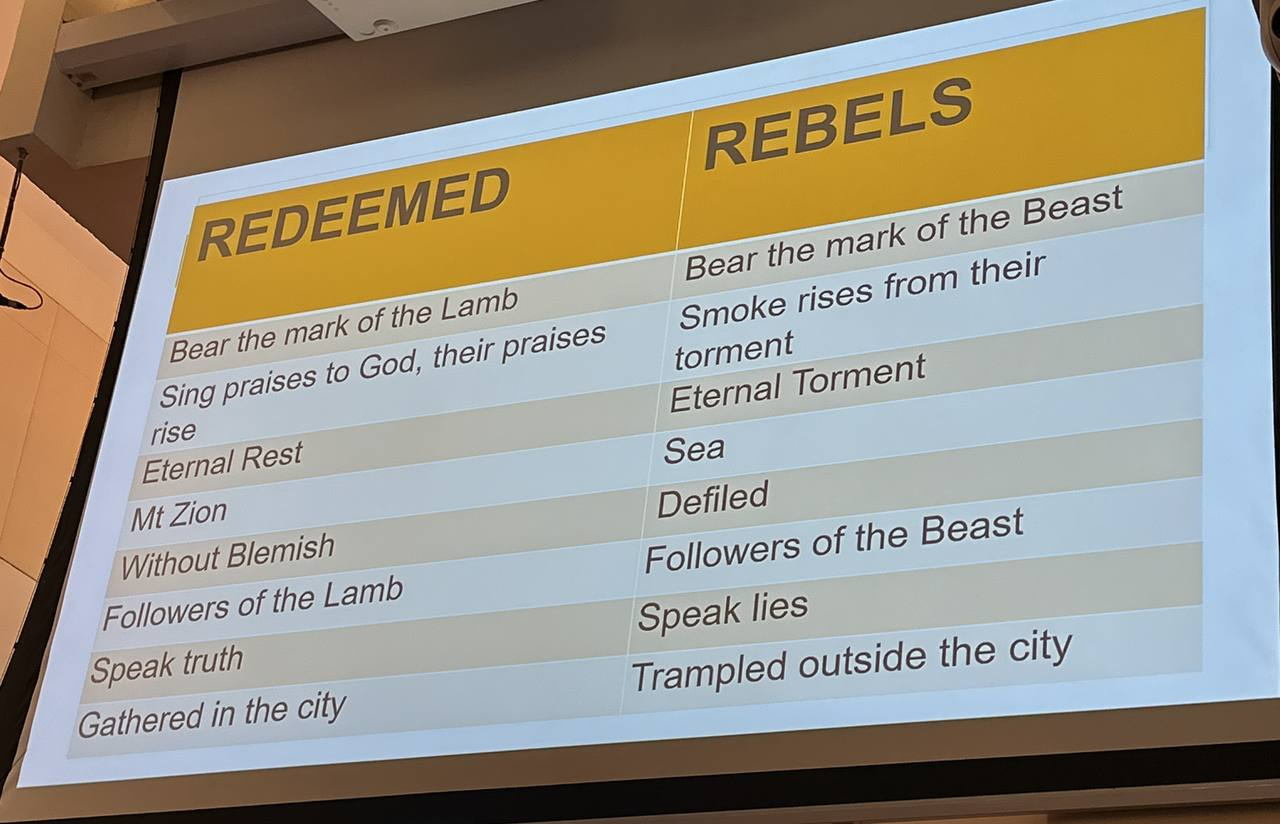
\includegraphics[width=0.8\textwidth, trim={0cm 0cm 0cm 0cm},clip]{Figures/marSermon3Fig1}
    \caption[]{Summary of the differences between the redeemed and the rebels}
    \label{}
  \end{figure}}
\end{itemize}